\subsection{Spectre on AMD and Intel}
Spectre attack works with high accuracy on AMD processors (we tried on Zen 3), but is extremely noisy on Alder Lake. While mistraining the branch predictor, pseudo-random access pattern is used to stop prefetcher from detecting it. But prefetcher present on Alder Lake is still able to detect this access pattern and prefetches the secret bytes even before they are speculatively brought into cache. This leads to very high noise in the attack.
\begin{figure}[H]
    \centering
    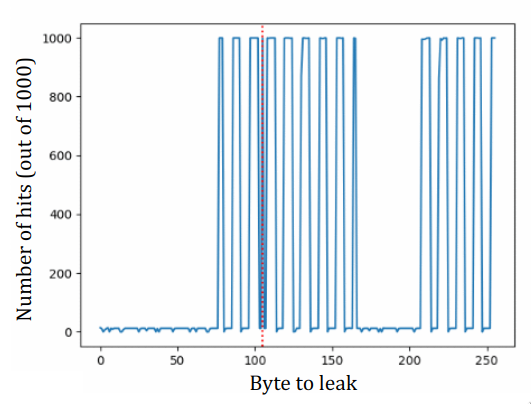
\includegraphics[width=0.4\textwidth]{images/giff.png}
    \caption{Detection of secret bytes on Alder Lake}
    \label{gif}
\end{figure}
\indent In the above figure \ref{gif}, Y-axis denotes the number of times the byte was detected out of 1000 iterations. X-axis denotes the byte number. Red dotted line denoted the secret byte that we want to leak. We can see that a peak is present on the red line, denoting that the secret byte is being detected. But at the same time lot of other bytes are also being detected. This is the noise present in the attack. This noise is very high on Alder Lake because of its prefetcher.

\subsection{RDTSC binning}
\indent We also found out that RDTSC on Zen 3 processors always returns the value which is a multiple of 32 or 33. AMD might have implemented binning of RDTSC to avoid timing attacks on its processors. Intel processors show no suggestion of such a binning being implemented.

\subsection{Flush variables involved in speculation}
\indent While carrying out spectre attack, in the speculative condition of \texttt{if(x < array\_size)}, it is necessary to ensure that the line corresponding to \texttt{array\_size} is not present in cache hierarchy. This ensures that the transient instructions have enought time to load the secret memory into cache hierarchy before they are squashed. Although hard to verify, this observation also hints towards the fact that the transient instructions are squashed as soon as the branch condition result is obtained. Processor does not wait for these transient instructions to reach the head of Reorder Buffer before squashing them.

\subsection{Branch Predictor}
\indent While mistraining the branch predictor on Haswell, we unrolled the for loop so that the victim function gets called by different instruction pointers. Spectre attack accuracy dropped massively after doing this. Branch predictor was not getting mistrained due to victim function being called by different instruction pointers. This shows us that branch predictor likely maintains a history of instruction pointers from which the victim function was called. Having different instruction pointers likely causes this history to get fuzzy leading to branch predictor not getting mistrained.

\subsection{Prime and Probe using linked list}
\indent We also tried prime and probe attack without using linked list. Instead we used memory fences to ensure that the next memory access happens after the previous access in completed. But this approach does not work, likely due to memory fences adding heavy overloads of their own leading to wrong timing measurements. Linked lists naturally ensure that the next memory access happens after the previous access is completed due to their structure. Thus, using linked lists for prime and probe is superior to using memory fences. \\
